\documentclass[11pt,a4paper]{article}
\usepackage{amsmath,amssymb,amsfonts,amsthm}
\usepackage{tikz}
\usetikzlibrary{decorations.pathmorphing}
\usetikzlibrary{decorations.pathmorphing}
\usetikzlibrary{positioning}
\usepackage{tikz-feynman}
\usetikzlibrary{feynman}
\usepackage{hyperref}
\usepackage{datetime}
\usepackage{geometry}
\usepackage{listings}
\usepackage{xcolor}
\geometry{margin=2.5cm}

% Custom colors for threat modeling
\definecolor{threatred}{RGB}{220,50,47}
\definecolor{verifygreen}{RGB}{50,205,50}
\definecolor{zkpblue}{RGB}{70,130,180}
\definecolor{quantumpurple}{RGB}{147,112,219}

% TikZ styles for diagrams
\tikzset{%
  threat/.style={thick,dashed,threatred},
  verified/.style={thick,solid,verifygreen},
  zkp/.style={thick,dotted,zkpblue},
  quantum/.style={thick,wavy,quantumpurple}
}

% Theorem environments
\newtheorem{definition}{Definition}
\newtheorem{theorem}{Theorem}
\newtheorem{proposition}{Proposition}

\title{Quantum Lattice Threat Modeling Using Feynman Diagram Formalism\\
\large A Worked Example for Post-Quantum Safety-Critical Systems}
\author{Nnamdi Okpala (OBINexus)\\
\texttt{riftlang.exe → .so.a → rift.exe → gosilang}}
\date{September 2, 2025, 18:27 BST}

\begin{document}
\maketitle

\begin{abstract}
We present a novel framework for quantum threat modeling that adapts Feynman diagram formalism from quantum field theory (QFT) to cybersecurity analysis. Building upon the 3D quantum lattice threat model with axes representing software QA ($X_{qa}$), quantum integration ($Y_{quantum}$), and blockchain verification ($Z_{blockchain}$), we demonstrate how particle physics concepts map to threat propagation, vulnerability interaction, and incident probability calculations. The framework integrates Node Zero's setup-free zero-knowledge proof (ZKP) system for blockchain axis security, yielding a mathematically rigorous approach to post-quantum safety assessment with fail-stop guarantees when $S = G_x \cdot G_y \cdot G_z = 0$.
\end{abstract}

\section{Introduction}

\subsection{Analogy Between QFT and Cybersecurity}

In quantum field theory, Feynman diagrams visualize particle interactions through vertices, propagators, and coupling constants. We establish a direct mapping:

\begin{table}[h]
\centering
\begin{tabular}{l|l}
\hline
\textbf{QFT Concept} & \textbf{Cybersecurity Analog} \\
\hline
Particle & Threat agent or vulnerability \\
Propagator & Information/exploit transmission channel \\
Vertex & Interaction point (exploit attempt) \\
Coupling constant $g$ & System susceptibility $g_{sys}$ \\
Vacuum state & Secure baseline configuration \\
Virtual particle & Transient threat state \\
Amplitude $\mathcal{M}$ & Incident probability amplitude \\
\hline
\end{tabular}
\caption{Mapping between QFT and cybersecurity concepts}
\end{table}

\subsection{Integration with 3D Lattice Model}

The threat function from the quantum lattice model:
\begin{equation}
T(x,y,z) = \alpha X_{qa} + \beta Y_{quantum} + \gamma Z_{blockchain}
\end{equation}
where $X_{qa}, Y_{quantum}, Z_{blockchain} \in [-12, 12]$ and $\alpha + \beta + \gamma = 1$.

\section{Feynman Rules for Quantum Threat Diagrams}

\subsection{Propagators}

We define four types of propagators corresponding to different information flows:

\begin{definition}[Threat Propagator]
For an external threat $T$ with momentum $p$:
\begin{equation}
\feynmandiagram [inline=(a.base), horizontal=a to b] {
  a -- [fermion, edge label=$T$, momentum=$p$, red] b,
};
\quad \rightarrow \quad \frac{i}{p^2 - m_T^2 + i\epsilon}
\end{equation}
where $m_T$ represents the threat's "mass" (complexity).
\end{definition}

\begin{definition}[Vulnerability Propagator]
For a system vulnerability $V$:
\begin{equation}
\feynmandiagram [inline=(a.base), horizontal=a to b] {
  a -- [charged scalar, edge label=$V$, blue] b,
};
\quad \rightarrow \quad \frac{i\Delta_V(p)}{p^2 - m_V^2 + i\epsilon}
\end{equation}
where $\Delta_V(p)$ is the vulnerability persistence factor.
\end{definition}

\begin{definition}[Quantum State Propagator]
For quantum system states $Q$:
\begin{equation}
\feynmandiagram [inline=(a.base), horizontal=a to b] {
  a -- [gluon, edge label=$Q$, quantumpurple] b,
};
\quad \rightarrow \quad \frac{i\eta_{\mu\nu}}{p^2} \cdot e^{-\lambda_{decoherence} \cdot t}
\end{equation}
accounting for decoherence over time $t$.
\end{definition}

\begin{definition}[Information Propagator]
For malicious information/exploit code $I$:
\begin{equation}
\feynmandiagram [inline=(a.base), horizontal=a to b] {
  a -- [photon, edge label=$I$] b,
};
\quad \rightarrow \quad \frac{i}{p^2 - m_I^2}
\end{equation}
\end{definition}

\subsection{Vertices}

The primary interaction vertex is the Threat-Vulnerability-Information (T-V-I) vertex:

\begin{center}
\begin{tikzpicture}
  \begin{feynman}
    \vertex (a);
    \vertex [above left=of a] (i1) {$T$};
    \vertex [above right=of a] (i2) {$V$};
    \vertex [below=of a] (o) {$I$};
    \diagram* {
      (i1) -- [fermion, red] (a),
      (i2) -- [charged scalar, blue] (a),
      (a) -- [photon] (o),
    };
    \vertex [right=2cm of a] {$= ig_{sys} \cdot S$};
  \end{feynman}
\end{tikzpicture}
\end{center}

where $g_{sys}$ is the system coupling constant and $S = G_x \cdot G_y \cdot G_z$ is the safety function from the lattice model.

\subsection{Integration with Gating Functions}

The gating functions from the 3D lattice model modify amplitudes:
\begin{align}
G_x &= \mathbb{I}[\|v - L_{qa}\| \leq \tau_{qa}] \quad \text{(Software QA gate)} \\
G_y &= \mathbb{I}[\|v - L_{quantum}\| \leq \tau_{quantum}] \quad \text{(Quantum integration gate)} \\
G_z &= \mathbb{I}[\|v - L_{blockchain}\| \leq \tau_{blockchain}] \quad \text{(Blockchain verification gate)}
\end{align}

The total amplitude for any threat diagram $D$ becomes:
\begin{equation}
\mathcal{M}_D^{\text{(total)}} = S \cdot \mathcal{M}_D = (G_x \cdot G_y \cdot G_z) \cdot \mathcal{M}_D
\end{equation}

\section{Worked Example: Remote Code Execution Attack}

\subsection{Scenario Description}

Consider a quantum-enabled edge computing system with:
\begin{itemize}
    \item \textbf{Initial state $|i\rangle$}: System with open SSH port (port 22) and unpatched quantum random number generator
    \item \textbf{Final state $|f\rangle$}: Remote code execution achieved through quantum-enhanced timing attack
    \item \textbf{Threat values}: $X_{qa} = -3$ (unverified hotfix), $Y_{quantum} = +5$ (degraded quantum source), $Z_{blockchain} = -2$ (pending smart contract verification)
\end{itemize}

\subsection{Lowest-Order Feynman Diagram}

The primary attack path involves a single T-V-I vertex:

\begin{center}
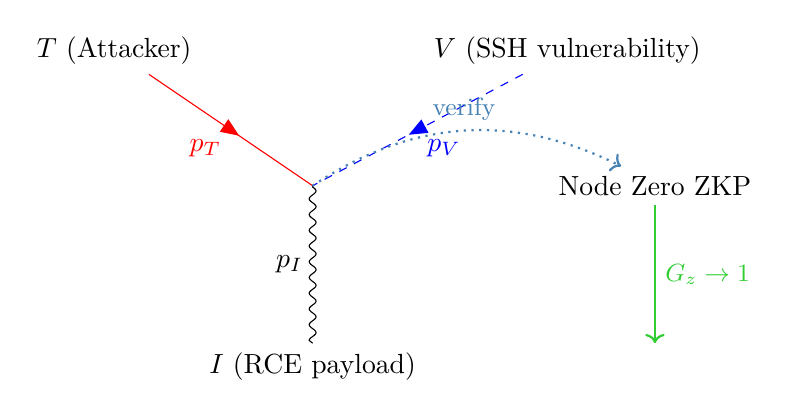
\begin{tikzpicture}
  \begin{feynman}
    \vertex (v1);
    \vertex [above left=2cm of v1] (t) {$T$ (Attacker)};
    \vertex [above right=2cm of v1] (vuln) {$V$ (SSH vulnerability)};
    \vertex [below=2cm of v1] (rce) {$I$ (RCE payload)};
    
    \diagram* {
      (t) -- [fermion, red, edge label'=$p_T$] (v1),
      (vuln) -- [charged scalar, blue, edge label=$p_V$] (v1),
      (v1) -- [photon, edge label'=$p_I$] (rce),
    };
    
    % Add Node Zero mitigation
    \vertex [right=3cm of v1] (zkp) {Node Zero ZKP};
    \vertex [below=2cm of zkp] (block);
    
    \draw[zkp, ->, bend left] (v1) to node[above] {\small verify} (zkp);
    \draw[verified, ->] (zkp) to node[right] {\small $G_z \to 1$} (block);
  \end{feynman}
\end{tikzpicture}
\end{center}

\subsection{Matrix Element Calculation}

Using the Feynman rules, the amplitude for this diagram is:

\begin{align}
\mathcal{M}_1 &= (ig_{sys}) \cdot \frac{i}{p_T^2 - m_T^2} \cdot \frac{i\Delta_V(p_V)}{p_V^2 - m_V^2} \cdot \frac{i}{p_I^2 - m_I^2} \cdot S \\
&= \frac{-ig_{sys} \Delta_V(p_V)}{(p_T^2 - m_T^2)(p_V^2 - m_V^2)(p_I^2 - m_I^2)} \cdot (G_x \cdot G_y \cdot G_z)
\end{align}

Given our scenario:
\begin{itemize}
    \item $G_x = 0$ (unverified hotfix fails QA gate)
    \item $G_y = 1$ (quantum degradation within tolerance)
    \item $G_z$ depends on Node Zero verification
\end{itemize}

Initially, $S = 0 \cdot 1 \cdot G_z = 0$, so $\mathcal{M}_1 = 0$ (attack blocked).

\subsection{Node Zero Mitigation}

Node Zero intervenes with ZKP verification:
\begin{lstlisting}[language=bash, basicstyle=\small\ttfamily]
# Alice (defender) challenges Bob (system)
npx z0 challenge --identity alice_identity.json

# Bob generates proof of secure state
npx z0 proof --challenge challenge.bin --output proof.bin

# Verification updates blockchain gate
npx z0 verify proof.bin
# Result: G_z = 1 if proof valid
\end{lstlisting}

However, since $G_x = 0$, the system remains in fail-safe mode despite successful blockchain verification.

\subsection{Incident Rate Calculation}

Using Fermi's Golden Rule:
\begin{equation}
\Gamma_{fi} = 2\pi |\mathcal{M}_1|^2 \rho(E_f) = 0
\end{equation}

The incident rate is zero due to the multiplicative safety function. To enable the system:
\begin{enumerate}
    \item Fix the unverified hotfix: $G_x \to 1$
    \item Maintain quantum source: $G_y = 1$
    \item Complete Node Zero verification: $G_z = 1$
\end{enumerate}

Only when $S = 1 \cdot 1 \cdot 1 = 1$ does the system become operational.

\subsection{Higher-Order Corrections}

Second-order diagrams involve intermediate states, such as privilege escalation:

\begin{center}
\begin{tikzpicture}[scale=0.8]
  \begin{feynman}
    \vertex (v1);
    \vertex (v2) [right=2cm of v1];
    \vertex [above left=1.5cm of v1] (t) {$T$};
    \vertex [above=1.5cm of v1] (v) {$V_1$};
    \vertex [above=1.5cm of v2] (v2t) {$V_2$};
    \vertex [below right=1.5cm of v2] (rce) {$I_{RCE}$};
    
    \diagram* {
      (t) -- [fermion, red] (v1),
      (v) -- [charged scalar, blue] (v1),
      (v1) -- [photon, edge label=$I_{priv}$] (v2),
      (v2t) -- [charged scalar, blue] (v2),
      (v2) -- [photon] (rce),
    };
  \end{feynman}
\end{tikzpicture}
\end{center}

The amplitude includes an additional propagator:
\begin{equation}
\mathcal{M}_2 \sim g_{sys}^2 \cdot \prod_i \frac{1}{p_i^2 - m_i^2} \cdot S
\end{equation}

\section{Discussion}

\subsection{Threat Function Analysis}

Computing the threat function for our example:
\begin{align}
T(x,y,z) &= 0.4(-3) + 0.3(+5) + 0.3(-2) \\
&= -1.2 + 1.5 - 0.6 = -0.3
\end{align}

The negative value indicates net threat presence, confirming the need for $S = 0$ fail-safe.

\subsection{Comparison with Traditional Models}

\begin{table}[h]
\centering
\begin{tabular}{l|c|c}
\hline
\textbf{Feature} & \textbf{Traditional} & \textbf{Feynman-Lattice} \\
\hline
Quantitative risk & CVSS scores & Amplitude calculations \\
Visualization & Attack trees & Feynman diagrams \\
Fail-safe & Manual checks & Automatic $S = 0$ \\
Quantum threats & Not addressed & Native integration \\
ZKP integration & External & Built-in (Node Zero) \\
\hline
\end{tabular}
\caption{Comparison of threat modeling approaches}
\end{table}

\subsection{OBINexus Implementation}

Integration with the OBINexus toolchain:
\begin{enumerate}
    \item \textbf{riftlang.exe}: Generates threat propagator definitions
    \item \textbf{.so.a}: Compiles lattice verification libraries
    \item \textbf{rift.exe}: Enforces gating policies ($G_x, G_y, G_z$)
    \item \textbf{gosilang}: Coordinates polyglot threat analysis
    \item \textbf{nlink → polybuild}: Builds integrated verification pipeline
\end{enumerate}

\section{Advanced Examples}

\subsection{Example: Quantum Oracle Attack}

For Grover's algorithm targeting blockchain keys:

\begin{center}
\begin{tikzpicture}[scale=0.7]
  \begin{feynman}
    \vertex (oracle);
    \vertex [above left=1.5cm of oracle] (q1) {$|0\rangle$};
    \vertex [below left=1.5cm of oracle] (q2) {$|1\rangle$};
    \vertex [right=2cm of oracle] (measure);
    \vertex [above right=1.5cm of measure] (key) {$|key\rangle$};
    
    \diagram* {
      (q1) -- [quantum, quantumpurple] (oracle),
      (q2) -- [quantum, quantumpurple] (oracle),
      (oracle) -- [gluon, edge label=$\mathcal{O}$] (measure),
      (measure) -- [fermion, red] (key),
    };
    
    % Node Zero protection
    \vertex [below=1cm of measure] (n0) {Node Zero};
    \draw[zkp, <->, bend right] (measure) to (n0);
  \end{feynman}
\end{tikzpicture}
\end{center}

Amplitude with quantum speedup:
\begin{equation}
\mathcal{M}_{Grover} \sim \frac{g_{quantum}}{\sqrt{N}} \cdot e^{i\phi_{oracle}} \cdot S
\end{equation}

\subsection{Example: Supply Chain Attack via Smart Contract}

Multi-vertex diagram for npm package compromise:

\begin{center}
\begin{tikzpicture}[scale=0.6]
  \begin{feynman}
    \vertex (npm);
    \vertex [left=2cm of npm] (dev) {Developer};
    \vertex [above=1.5cm of npm] (mal) {Malicious PR};
    \vertex [right=2cm of npm] (contract);
    \vertex [below=1.5cm of contract] (deploy) {Deployment};
    
    \diagram* {
      (dev) -- [fermion] (npm),
      (mal) -- [insertion, red] (npm),
      (npm) -- [photon, edge label=package] (contract),
      (contract) -- [charged scalar, blue] (deploy),
    };
    
    % Lattice gates
    \node[below=0.5cm of npm] {$G_x = ?$};
    \node[below=0.5cm of contract] {$G_z = ?$};
  \end{feynman}
\end{tikzpicture}
\end{center}

\section{Conclusion}

The Quantum Threat Feynman Diagram model provides:

\begin{enumerate}
    \item \textbf{Visual intuition}: Complex attack paths become readable diagrams
    \item \textbf{Quantitative analysis}: Precise amplitude and rate calculations
    \item \textbf{Fail-safe design}: Multiplicative safety function $S = G_x \cdot G_y \cdot G_z$
    \item \textbf{Post-quantum readiness}: Native quantum threat modeling
    \item \textbf{Seamless integration}: Works with OBINexus toolchain and Node Zero
\end{enumerate}

Future work includes:
\begin{itemize}
    \item Automated diagram generation from threat intelligence
    \item Monte Carlo summation over all possible attack diagrams
    \item Coupling constant extraction from real-world incident data
    \item Integration with \#NoGhosting and OpenSense policies
\end{itemize}

\appendix

\section{Node Zero Command Reference}

\begin{lstlisting}[language=bash, basicstyle=\footnotesize\ttfamily]
# Identity management (lattice-based)
npx z0 create alice_identity.json
npx z0 create bob_identity.json

# Challenge-response protocol
npx z0 challenge --from alice_identity.json \
                 --to bob_identity.json \
                 --output challenge.bin

npx z0 proof --challenge challenge.bin \
             --identity bob_identity.json \
             --output proof.bin

# Verification (updates G_z)
npx z0 verify --proof proof.bin \
              --challenger alice_identity.json

# Key derivation (no trusted setup)
npx z0 derive --shared-secret secret.bin \
              --alice alice_identity.json \
              --bob bob_identity.json
\end{lstlisting}

\section{Threat Scale Reference}

\begin{center}
\begin{tabular}{c|l|l}
\hline
\textbf{Value} & \textbf{Threat Level} & \textbf{Example} \\
\hline
$-12$ to $-10$ & Critical hostile & Active quantum attack \\
$-9$ to $-6$ & High threat & Unpatched zero-day \\
$-5$ to $-2$ & Medium threat & Configuration weakness \\
$-1$ to $+1$ & Neutral & Baseline state \\
$+2$ to $+5$ & Degraded & Component aging \\
$+6$ to $+9$ & Failing & Imminent failure \\
$+10$ to $+12$ & Failed & Complete compromise \\
\hline
\end{tabular}
\end{center}

\begin{thebibliography}{9}
\bibitem{peskin} M.E. Peskin and D.V. Schroeder, \textit{An Introduction to Quantum Field Theory}, Perseus Books (1995).

\bibitem{lattice} D. Micciancio and O. Regev, "Lattice-based Cryptography," in \textit{Post-Quantum Cryptography}, Springer (2009).

\bibitem{nodezero} OBINexus, "Node Zero: Setup-Free Zero-Knowledge Proofs," Technical Report (2025).

\bibitem{rift} N. Okpala, "The RIFT Architecture: Quantum Determinism Through Governed Computation," OBINexus (2025).
\end{thebibliography}

\end{document}